%%%%%%%%%%%%%%%%%%%%%%%%%%%%%%%%%%%%%%%%%
% Beamer Presentation
% LaTeX Template
% Version 1.0 (10/11/12)
%
% This template has been downloaded from:
% http://www.LaTeXTemplates.com
%
% License:
% CC BY-NC-SA 3.0 (http://creativecommons.org/licenses/by-nc-sa/3.0/)
%
%%%%%%%%%%%%%%%%%%%%%%%%%%%%%%%%%%%%%%%%%

%----------------------------------------------------------------------------------------
%	PACKAGES AND THEMES
%----------------------------------------------------------------------------------------

\documentclass{beamer}

\mode<presentation> {

% The Beamer class comes with a number of default slide themes
% which change the colors and layouts of slides. Below this is a list
% of all the themes, uncomment each in turn to see what they look like.

%\usetheme{default}
%\usetheme{AnnArbor}
%\usetheme{Antibes}
%\usetheme{Bergen}
%\usetheme{Berkeley}
%\usetheme{Berlin}
%\usetheme{Boadilla}
%\usetheme{CambridgeUS}
%\usetheme{Copenhagen}
%\usetheme{Darmstadt}
%\usetheme{Dresden}
%\usetheme{Frankfurt}
%\usetheme{Goettingen}
%\usetheme{Hannover}
%\usetheme{Ilmenau}
%\usetheme{JuanLesPins}
%\usetheme{Luebeck}
%\usetheme{Madrid}
\usetheme{htw}
%\usetheme{Malmoe}
%\usetheme{Marburg}
%\usetheme{Montpellier}
%\usetheme{PaloAlto}
%\usetheme{Pittsburgh}
%\usetheme{Rochester}
%\usetheme{Singapore}
%\usetheme{Szeged}
%\usetheme{Warsaw}

% As well as themes, the Beamer class has a number of color themes
% for any slide theme. Uncomment each of these in turn to see how it
% changes the colors of your current slide theme.

%\usecolortheme{albatross}
%\usecolortheme{beaver}
%\usecolortheme{beetle}
%\usecolortheme{crane}
%\usecolortheme{dolphin}
%\usecolortheme{dove}
%\usecolortheme{fly}
%\usecolortheme{lily}
%\usecolortheme{orchid}
%\usecolortheme{rose}
%\usecolortheme{seagull}
%\usecolortheme{seahorse}
%\usecolortheme{whale}
%\usecolortheme{wolverine}

%\setbeamertemplate{footline} % To remove the footer line in all slides uncomment this line
%\setbeamertemplate{footline}[page number] % To replace the footer line in all slides with a simple slide count uncomment this line

%\setbeamertemplate{navigation symbols}{} % To remove the navigation symbols from the bottom of all slides uncomment this line
}

\usepackage{graphicx} % Allows including images
\usepackage{booktabs} % Allows the use of \toprule, \midrule and \bottomrule in tables
\usepackage{amsmath}
\usepackage{algorithm}
\usepackage[noend]{algpseudocode}

\makeatletter
\def\BState{\State\hskip-\ALG@thistlm}
\makeatother

%----------------------------------------------------------------------------------------
%	TITLE PAGE
%----------------------------------------------------------------------------------------

\title[Radixsort MPI]{Paralleler Radixsort MPI} % The short title appears at the bottom of every slide, the full title is only on the title page

\author{Steffen Bohr, Marcus Kl\"usener} % Your name
\institute[HTW-Berlin] % Your institution as it will appear on the bottom of every slide, may be shorthand to save space
{
HTW-Berlin \\ % Your institution for the title page
\medskip
%\textit{john@smith.com} % Your email address
}
\date{\today} % Date, can be changed to a custom date

\begin{document}

\begin{frame}
\titlepage % Print the title page as the first slide
\end{frame}

\begin{frame}
\frametitle{\"Ubersicht} % Table of contents slide, comment this block out to remove it
\tableofcontents % Throughout your presentation, if you choose to use \section{} and \subsection{} commands, these will automatically be printed on this slide as an overview of your presentation
\end{frame}

%----------------------------------------------------------------------------------------
%	PRESENTATION SLIDES
%----------------------------------------------------------------------------------------

%------------------------------------------------
\section{SF-Radix Sort} % Sections can be created in order to organize your presentation into discrete blocks, all sections and subsections are automatically printed in the table of contents as an overview of the talk
%------------------------------------------------

\subsection{Pseudocode} % A subsection can be created just before a set of slides with a common theme to further break down your presentation into chunks

\begin{frame}
\frametitle{Distributed memory SF-Radix Sort 1/2}
\begin{algorithmic}[1]
\For{dig = least significant digit \textbf{to} most significant digit}  
	\State initialize (LC, nbuckets)
	\For{i=0 \textbf{to} N-1} 
		\State value = get\_digit\_value(S[i],dig)
		\State LC[value] = LC[value]+1
	\EndFor
	\State tmp = LC[0]
	\State LC[0] = 0

	\For{i=1 \textbf{to} nbuckets-1}
		\State accum = tmp+LC[i-1]
		\State tmp = LC[i]
		\State LC[i] = accum
	\EndFor
	\algstore{myalg}
\end{algorithmic}
\end{frame}

%------------------------------------------------

\begin{frame}
\frametitle{Distributed memory SF-Radix Sort 2/2}
\begin{algorithmic}[1]
	\algrestore{myalg}
	\For{i=0 \textbf{to} N-1}
		\State value=get\_digit\_value(S[i],dig)
		\State D[LC[value]] = S[i]
		\State LC[value] = LC[value]+1
	\EndFor
	\State Gl[pid][0] = LC[0]
	\For{i=1 \textbf{to} nbuckets-1}
		\State Gl[pid][i] = LC[i]-LC[i-1]
	\EndFor
	\State \textbf{allgather}(Gl[pid][0], nbuckets, Gl)
	\State \textbf{bucketdistribution}(Gl)
	\State \textbf{datacommunication}(S, D,Gl)
	\State \textbf{swapaddresses}(S, D)
\EndFor
\end{algorithmic}
\end{frame}

%------------------------------------------------
\subsection{Beispieliterationen}
\begin{frame}
	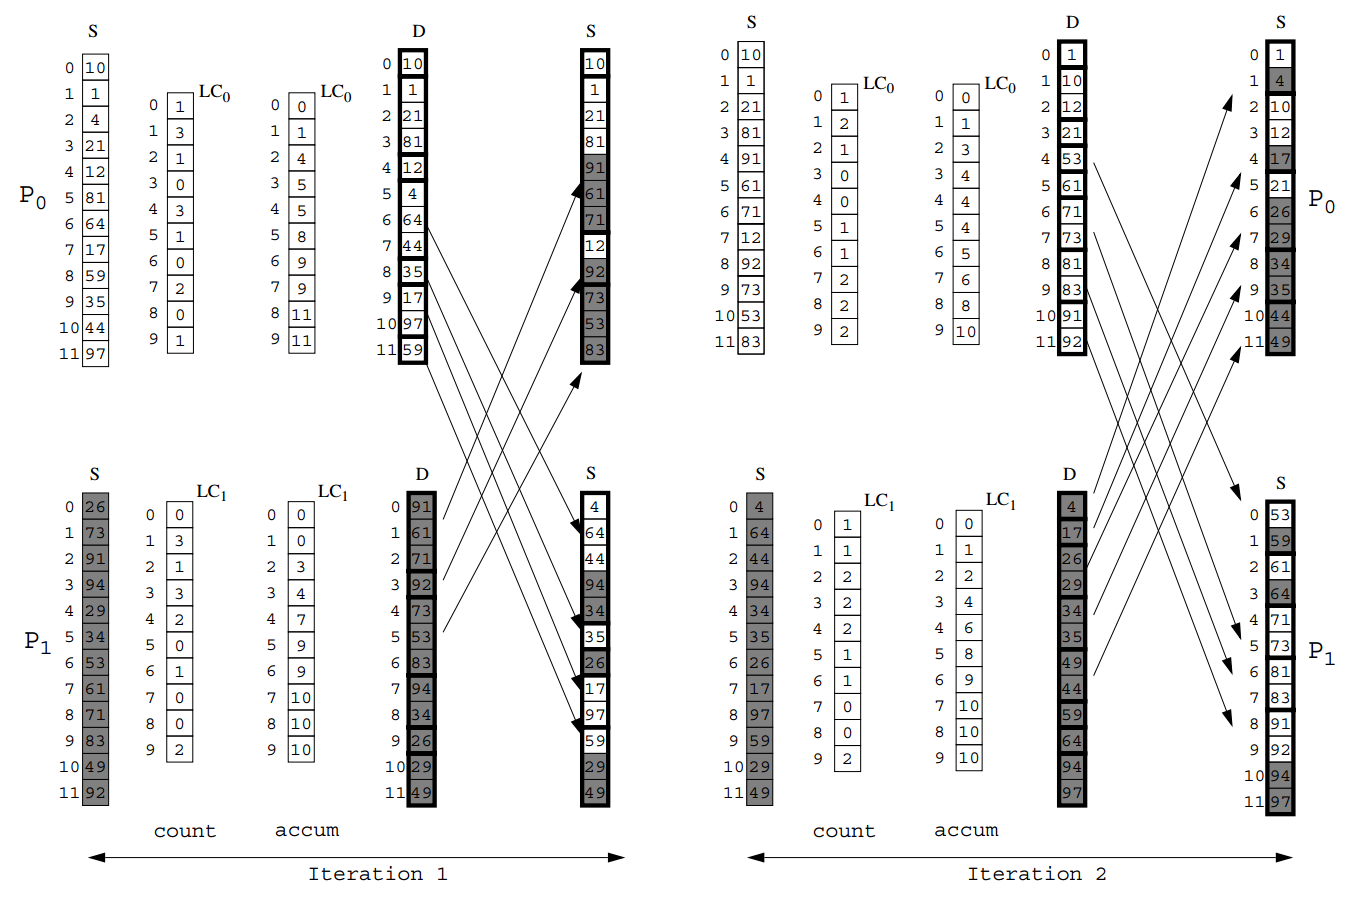
\includegraphics[width=\textwidth]{SF-RadixIteration.png}
\end{frame}

%------------------------------------------------
\section{C3-Radix Sort}
%------------------------------------------------

\begin{frame}
\frametitle{C3-Radix Sort Ablauf}
\begin{itemize}
\item Jeder Prozessort initialisiert seine Counter und die globale Countermatrix.
\item Erzeugt ein Histogram aus den Zeichen mit der h\"ochsten Wertigkeit aller lokalen Schl\"ussel.
\item Berechnet die lokale Akkumulation mit Hilfe der globalen Countermatrix.
\item Sortiert die lokalen Schl\"ussel anhand der lokalen Akkumulation in Buckets.
\item Versendet die lokalen Buckets so das eine gleichmäßige Lastverteilung entsteht.
\item Wenn keine gleichm\"a\ss{}ige Lastverteilung entstehen w\"urde wird der ganze Sortiervorgang mit dem n\"achsten Zeichen wiederholt.
\item Jeder Prozessor sortiert seine Buckets nur noch lokal.
\end{itemize}
\end{frame}

%------------------------------------------------

\subsection{C3-Radix Sort Beispiel}
\begin{frame}
	\begin{figure}[ht]
	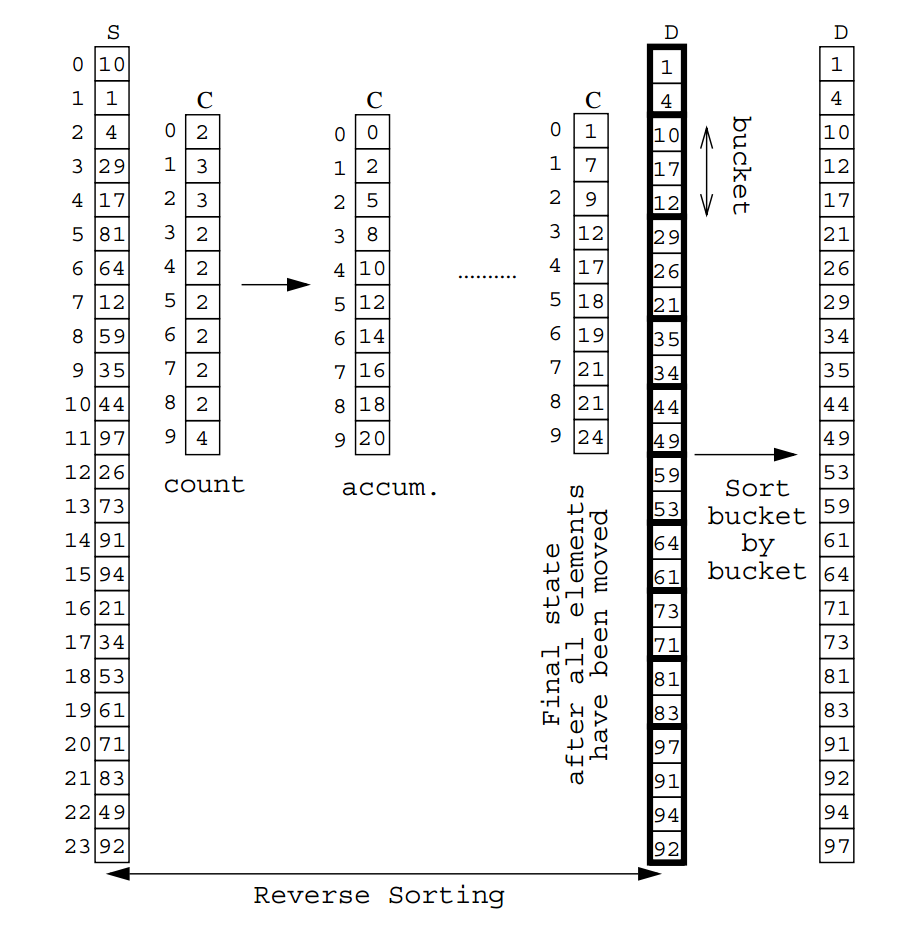
\includegraphics[width=200px]{C3RadixSort.png}
	\end{figure}
\end{frame}

%------------------------------------------------
\section{Herausforderungen}
%------------------------------------------------

\begin{frame}
\frametitle{Herausforderungen}
\begin{itemize}
\item Bucketgr\"o\ss{}e bei vielen gleichen Zeichen
\item Verteilung der Buckets
\end{itemize}
\end{frame}
\begin{frame}

%------------------------------------------------

\Huge{\centerline{Vielen Dank}}
\end{frame}

%----------------------------------------------------------------------------------------

\end{document} 
